\subsection{Decentralized Variance-Reduced SGF FW Experiments}
The experiments performed with Algorithm \ref{variance-reduced} were conducted considering $M=5$ workers. Each worker was fed with $S_1=800$ images (80 images per class) from the portion of the MNIST test set that LeNet5 was able to classify correctly. We imposed that the same image could not be assigned to different workers. This aspect was not clearly specified in the original algorithm proposed in \cite{A3}, section VI, in which the authors seem to suggest to use the same $S_1$ images for all the workers. However, the distributed data settings arise from the need of dividing huge datasets into different machines, for simplifying the computational complexity, and therefore we opted for an implementation choice that resulted more coherent with this idea.\\  \indent The number $M$ of workers was halved compared to the one of the previous algorithm and also the other hyperparameters was chosen to be pretty low to reduce a bit the CPU-time consumption. In particular, we set the number of component functions to $n=5$ or $n=10$, the number of sampled components in RDSA to $S_2=3$, the number of queries to $T=20$ and the period parameter to $q=5$ or $q=7$ or $q=9$. With these settings, the algorithm approximatively took between one and four hours to terminate. In fact, the algorithm combines the hungry but accurate queries of KWSA, regulated by the parameter $q$, with the efficient but potentially inaccurate queries of RDSA.\\
\indent In Table \ref{tab:vr} are reported the values of the accuracy reached by LeNet-5 with the adversarial examples obtained using the perturbation generated by Algorithm \ref{variance-reduced}. The attack seems to be more effective as the value of $q$ decreases, i.e. as the KWSA scheme is performed more frequently.\\
\begin{table}[htbp]
	\begin{center}
		\begin{adjustwidth}{-.6cm}{}
			\begin{tabular}{c|cccc}
				\textbf{Attack} &    &      q=5 &      q=7 &     q=10 \\
				\midrule
				{\small Decentralized Variance-}  & n=5   &    92,37\% &    97,43\% &       94,18\% \\
				{\small Reduced SGF FW}     &  n=10&  84,00\% &    93,66\% &       98,99\% \\
			\end{tabular}
		\end{adjustwidth}
	\end{center}
\caption{{\small Summary of $\ell_\infty$ Universal Adversarial Perturbation with $\varepsilon$=0.25. MNIST attacks using Decentralized Variance-Reduced SGF FW. The entries of the table represent the accuracies of LeNet-5 for the three different attacks. For increasing values of $q$ the algorithm performs the KWSA scheme less and less times.}}
	\label{tab:vr}
\end{table}

Figure \ref{fig:vred} compares two adversarial perturbations obtained with same $n$ but different values of $q$. It's clear that the perturbation computed with the lowest $q$ is smoother than the other and less visible to the human eyes.\\
\indent By looking at the colorbar, we can also observe that a higher $q$ results in higher absolute values of the perturbation's components: bright yellow and dark blue pixels indicate values near $\pm\varepsilon$ and are much more frequent in the perturbation computed with the highest $q$.

\begin{figure}[h]
	\begin{subfigure}[b]{0.15\textwidth}
		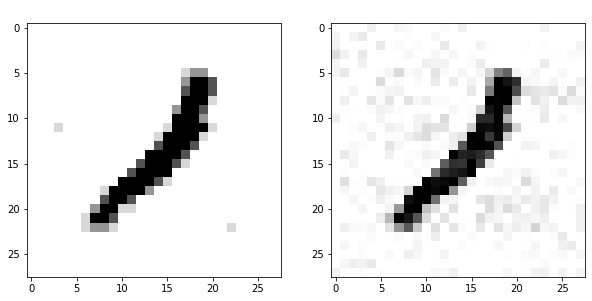
\includegraphics[width=5cm]{image_pertub_q5_n10_final.png}
	\end{subfigure}
	\hspace{2.5cm}
	\begin{subfigure}[b]{0.15\textwidth}
		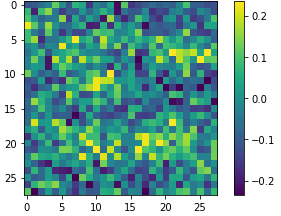
\includegraphics[width=3.08cm]{1.png}
	\end{subfigure}
	\newline
	\centerline{(a)}
	\begin{subfigure}[b]{0.15\textwidth}
		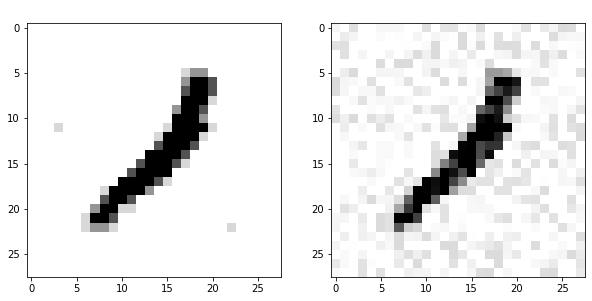
\includegraphics[width=5cm]{image_pertub_q10_n10_final.png}
	\end{subfigure}
	\hspace{2.5cm}
	\begin{subfigure}[b]{0.15\textwidth}
		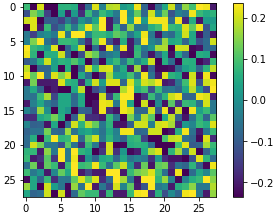
\includegraphics[width=3.07cm]{2.png}
	\end{subfigure}
	\newline
	\centerline{(b)}
	\caption{{\small (a) Adversarial example obtained from Algorithm \ref{variance-reduced} with $n=10$, $q=5$. (b) Adversarial example obtained from Algorithm \ref{variance-reduced} with $n=10$, $q=10$.}  }
	\label{fig:vred}
\end{figure}
